% Created by tikzDevice version 0.12.3.1 on 2022-10-05 10:09:10
% !TEX encoding = UTF-8 Unicode
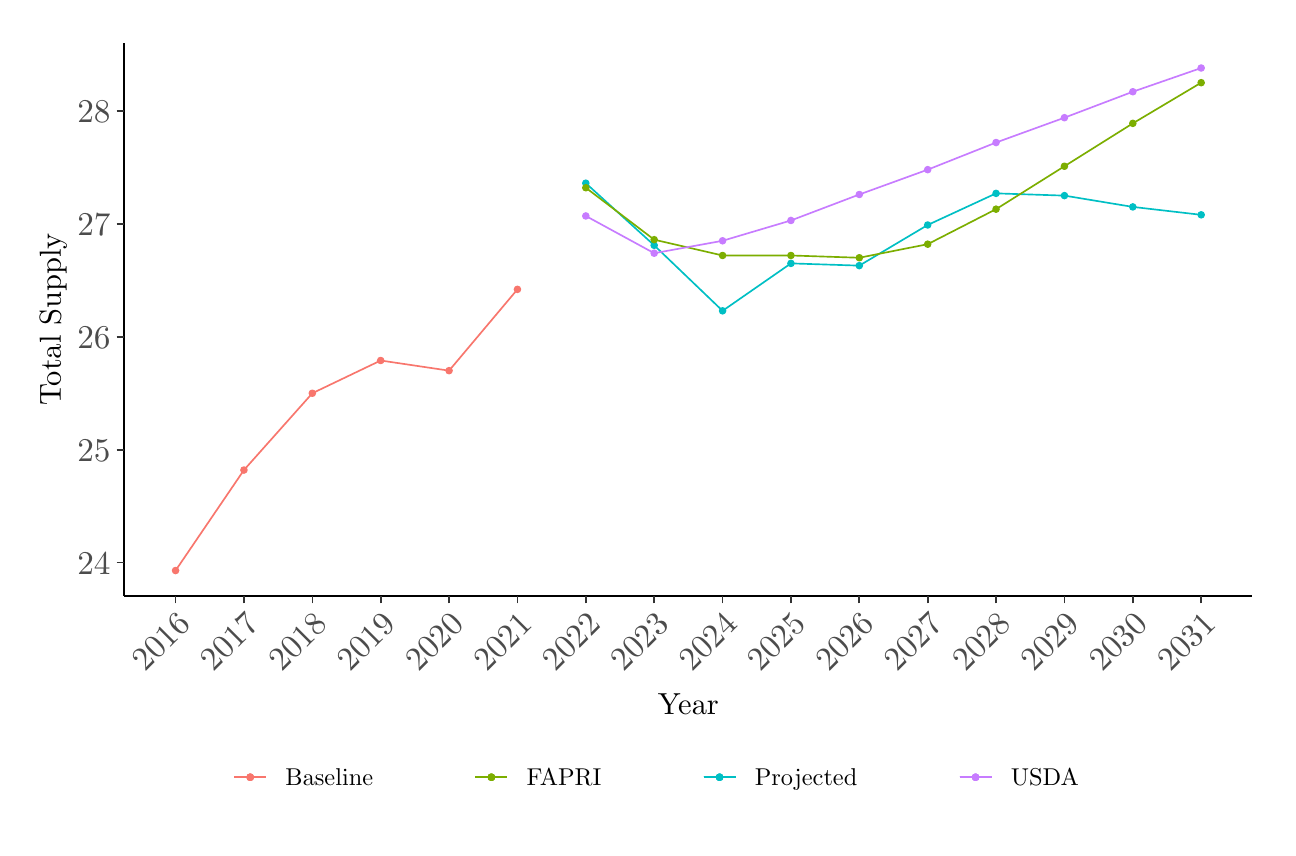
\begin{tikzpicture}[x=1pt,y=1pt]
\definecolor{fillColor}{RGB}{255,255,255}
\path[use as bounding box,fill=fillColor,fill opacity=0.00] (0,0) rectangle (448.07,289.08);
\begin{scope}
\path[clip] (  0.00,  0.00) rectangle (448.07,289.08);
\definecolor{drawColor}{RGB}{255,255,255}
\definecolor{fillColor}{RGB}{255,255,255}

\path[draw=drawColor,line width= 0.6pt,line join=round,line cap=round,fill=fillColor] (  0.00, -0.00) rectangle (448.07,289.08);
\end{scope}
\begin{scope}
\path[clip] ( 34.91, 83.83) rectangle (442.57,283.58);
\definecolor{fillColor}{RGB}{255,255,255}

\path[fill=fillColor] ( 34.91, 83.83) rectangle (442.57,283.58);
\definecolor{drawColor}{RGB}{248,118,109}

\path[draw=drawColor,line width= 0.6pt,line join=round] ( 53.44, 92.91) --
	( 78.15,129.23) --
	(102.86,156.98) --
	(127.56,168.81) --
	(152.27,165.14) --
	(176.98,194.52);
\definecolor{fillColor}{RGB}{248,118,109}

\path[draw=drawColor,line width= 0.4pt,line join=round,line cap=round,fill=fillColor] ( 53.44, 92.91) circle (  1.16);

\path[draw=drawColor,line width= 0.4pt,line join=round,line cap=round,fill=fillColor] ( 78.15,129.23) circle (  1.16);

\path[draw=drawColor,line width= 0.4pt,line join=round,line cap=round,fill=fillColor] (102.86,156.98) circle (  1.16);

\path[draw=drawColor,line width= 0.4pt,line join=round,line cap=round,fill=fillColor] (127.56,168.81) circle (  1.16);

\path[draw=drawColor,line width= 0.4pt,line join=round,line cap=round,fill=fillColor] (152.27,165.14) circle (  1.16);

\path[draw=drawColor,line width= 0.4pt,line join=round,line cap=round,fill=fillColor] (176.98,194.52) circle (  1.16);
\definecolor{drawColor}{RGB}{0,191,196}

\path[draw=drawColor,line width= 0.6pt,line join=round] (201.68,232.88) --
	(226.39,210.43) --
	(251.10,186.76) --
	(275.80,203.90) --
	(300.51,203.09) --
	(325.22,217.78) --
	(349.92,229.20) --
	(374.63,228.39) --
	(399.34,224.31) --
	(424.04,221.45);
\definecolor{fillColor}{RGB}{0,191,196}

\path[draw=drawColor,line width= 0.4pt,line join=round,line cap=round,fill=fillColor] (201.68,232.88) circle (  1.16);

\path[draw=drawColor,line width= 0.4pt,line join=round,line cap=round,fill=fillColor] (226.39,210.43) circle (  1.16);

\path[draw=drawColor,line width= 0.4pt,line join=round,line cap=round,fill=fillColor] (251.10,186.76) circle (  1.16);

\path[draw=drawColor,line width= 0.4pt,line join=round,line cap=round,fill=fillColor] (275.80,203.90) circle (  1.16);

\path[draw=drawColor,line width= 0.4pt,line join=round,line cap=round,fill=fillColor] (300.51,203.09) circle (  1.16);

\path[draw=drawColor,line width= 0.4pt,line join=round,line cap=round,fill=fillColor] (325.22,217.78) circle (  1.16);

\path[draw=drawColor,line width= 0.4pt,line join=round,line cap=round,fill=fillColor] (349.92,229.20) circle (  1.16);

\path[draw=drawColor,line width= 0.4pt,line join=round,line cap=round,fill=fillColor] (374.63,228.39) circle (  1.16);

\path[draw=drawColor,line width= 0.4pt,line join=round,line cap=round,fill=fillColor] (399.34,224.31) circle (  1.16);

\path[draw=drawColor,line width= 0.4pt,line join=round,line cap=round,fill=fillColor] (424.04,221.45) circle (  1.16);
\definecolor{drawColor}{RGB}{124,174,0}

\path[draw=drawColor,line width= 0.6pt,line join=round] (201.68,231.24) --
	(226.39,212.47) --
	(251.10,206.76) --
	(275.80,206.76) --
	(300.51,205.94) --
	(325.22,210.84) --
	(349.92,223.49) --
	(374.63,239.00) --
	(399.34,254.50) --
	(424.04,269.20);
\definecolor{fillColor}{RGB}{124,174,0}

\path[draw=drawColor,line width= 0.4pt,line join=round,line cap=round,fill=fillColor] (201.68,231.24) circle (  1.16);

\path[draw=drawColor,line width= 0.4pt,line join=round,line cap=round,fill=fillColor] (226.39,212.47) circle (  1.16);

\path[draw=drawColor,line width= 0.4pt,line join=round,line cap=round,fill=fillColor] (251.10,206.76) circle (  1.16);

\path[draw=drawColor,line width= 0.4pt,line join=round,line cap=round,fill=fillColor] (275.80,206.76) circle (  1.16);

\path[draw=drawColor,line width= 0.4pt,line join=round,line cap=round,fill=fillColor] (300.51,205.94) circle (  1.16);

\path[draw=drawColor,line width= 0.4pt,line join=round,line cap=round,fill=fillColor] (325.22,210.84) circle (  1.16);

\path[draw=drawColor,line width= 0.4pt,line join=round,line cap=round,fill=fillColor] (349.92,223.49) circle (  1.16);

\path[draw=drawColor,line width= 0.4pt,line join=round,line cap=round,fill=fillColor] (374.63,239.00) circle (  1.16);

\path[draw=drawColor,line width= 0.4pt,line join=round,line cap=round,fill=fillColor] (399.34,254.50) circle (  1.16);

\path[draw=drawColor,line width= 0.4pt,line join=round,line cap=round,fill=fillColor] (424.04,269.20) circle (  1.16);
\definecolor{drawColor}{RGB}{199,124,255}

\path[draw=drawColor,line width= 0.6pt,line join=round] (201.68,221.04) --
	(226.39,207.58) --
	(251.10,212.07) --
	(275.80,219.41) --
	(300.51,228.80) --
	(325.22,237.77) --
	(349.92,247.57) --
	(374.63,256.55) --
	(399.34,265.93) --
	(424.04,274.50);
\definecolor{fillColor}{RGB}{199,124,255}

\path[draw=drawColor,line width= 0.4pt,line join=round,line cap=round,fill=fillColor] (201.68,221.04) circle (  1.16);

\path[draw=drawColor,line width= 0.4pt,line join=round,line cap=round,fill=fillColor] (226.39,207.58) circle (  1.16);

\path[draw=drawColor,line width= 0.4pt,line join=round,line cap=round,fill=fillColor] (251.10,212.07) circle (  1.16);

\path[draw=drawColor,line width= 0.4pt,line join=round,line cap=round,fill=fillColor] (275.80,219.41) circle (  1.16);

\path[draw=drawColor,line width= 0.4pt,line join=round,line cap=round,fill=fillColor] (300.51,228.80) circle (  1.16);

\path[draw=drawColor,line width= 0.4pt,line join=round,line cap=round,fill=fillColor] (325.22,237.77) circle (  1.16);

\path[draw=drawColor,line width= 0.4pt,line join=round,line cap=round,fill=fillColor] (349.92,247.57) circle (  1.16);

\path[draw=drawColor,line width= 0.4pt,line join=round,line cap=round,fill=fillColor] (374.63,256.55) circle (  1.16);

\path[draw=drawColor,line width= 0.4pt,line join=round,line cap=round,fill=fillColor] (399.34,265.93) circle (  1.16);

\path[draw=drawColor,line width= 0.4pt,line join=round,line cap=round,fill=fillColor] (424.04,274.50) circle (  1.16);
\end{scope}
\begin{scope}
\path[clip] (  0.00,  0.00) rectangle (448.07,289.08);
\definecolor{drawColor}{RGB}{0,0,0}

\path[draw=drawColor,line width= 0.6pt,line join=round] ( 34.91, 83.83) --
	( 34.91,283.58);
\end{scope}
\begin{scope}
\path[clip] (  0.00,  0.00) rectangle (448.07,289.08);
\definecolor{drawColor}{gray}{0.30}

\node[text=drawColor,anchor=base east,inner sep=0pt, outer sep=0pt, scale=  1.20] at ( 29.96, 91.63) {24};

\node[text=drawColor,anchor=base east,inner sep=0pt, outer sep=0pt, scale=  1.20] at ( 29.96,132.44) {25};

\node[text=drawColor,anchor=base east,inner sep=0pt, outer sep=0pt, scale=  1.20] at ( 29.96,173.25) {26};

\node[text=drawColor,anchor=base east,inner sep=0pt, outer sep=0pt, scale=  1.20] at ( 29.96,214.05) {27};

\node[text=drawColor,anchor=base east,inner sep=0pt, outer sep=0pt, scale=  1.20] at ( 29.96,254.86) {28};
\end{scope}
\begin{scope}
\path[clip] (  0.00,  0.00) rectangle (448.07,289.08);
\definecolor{drawColor}{gray}{0.20}

\path[draw=drawColor,line width= 0.6pt,line join=round] ( 32.16, 95.76) --
	( 34.91, 95.76);

\path[draw=drawColor,line width= 0.6pt,line join=round] ( 32.16,136.57) --
	( 34.91,136.57);

\path[draw=drawColor,line width= 0.6pt,line join=round] ( 32.16,177.38) --
	( 34.91,177.38);

\path[draw=drawColor,line width= 0.6pt,line join=round] ( 32.16,218.19) --
	( 34.91,218.19);

\path[draw=drawColor,line width= 0.6pt,line join=round] ( 32.16,258.99) --
	( 34.91,258.99);
\end{scope}
\begin{scope}
\path[clip] (  0.00,  0.00) rectangle (448.07,289.08);
\definecolor{drawColor}{RGB}{0,0,0}

\path[draw=drawColor,line width= 0.6pt,line join=round] ( 34.91, 83.83) --
	(442.57, 83.83);
\end{scope}
\begin{scope}
\path[clip] (  0.00,  0.00) rectangle (448.07,289.08);
\definecolor{drawColor}{gray}{0.20}

\path[draw=drawColor,line width= 0.6pt,line join=round] ( 53.44, 81.08) --
	( 53.44, 83.83);

\path[draw=drawColor,line width= 0.6pt,line join=round] ( 78.15, 81.08) --
	( 78.15, 83.83);

\path[draw=drawColor,line width= 0.6pt,line join=round] (102.86, 81.08) --
	(102.86, 83.83);

\path[draw=drawColor,line width= 0.6pt,line join=round] (127.56, 81.08) --
	(127.56, 83.83);

\path[draw=drawColor,line width= 0.6pt,line join=round] (152.27, 81.08) --
	(152.27, 83.83);

\path[draw=drawColor,line width= 0.6pt,line join=round] (176.98, 81.08) --
	(176.98, 83.83);

\path[draw=drawColor,line width= 0.6pt,line join=round] (201.68, 81.08) --
	(201.68, 83.83);

\path[draw=drawColor,line width= 0.6pt,line join=round] (226.39, 81.08) --
	(226.39, 83.83);

\path[draw=drawColor,line width= 0.6pt,line join=round] (251.10, 81.08) --
	(251.10, 83.83);

\path[draw=drawColor,line width= 0.6pt,line join=round] (275.80, 81.08) --
	(275.80, 83.83);

\path[draw=drawColor,line width= 0.6pt,line join=round] (300.51, 81.08) --
	(300.51, 83.83);

\path[draw=drawColor,line width= 0.6pt,line join=round] (325.22, 81.08) --
	(325.22, 83.83);

\path[draw=drawColor,line width= 0.6pt,line join=round] (349.92, 81.08) --
	(349.92, 83.83);

\path[draw=drawColor,line width= 0.6pt,line join=round] (374.63, 81.08) --
	(374.63, 83.83);

\path[draw=drawColor,line width= 0.6pt,line join=round] (399.34, 81.08) --
	(399.34, 83.83);

\path[draw=drawColor,line width= 0.6pt,line join=round] (424.04, 81.08) --
	(424.04, 83.83);
\end{scope}
\begin{scope}
\path[clip] (  0.00,  0.00) rectangle (448.07,289.08);
\definecolor{drawColor}{gray}{0.30}

\node[text=drawColor,rotate= 45.00,anchor=base east,inner sep=0pt, outer sep=0pt, scale=  1.20] at ( 59.29, 73.03) {2016};

\node[text=drawColor,rotate= 45.00,anchor=base east,inner sep=0pt, outer sep=0pt, scale=  1.20] at ( 83.99, 73.03) {2017};

\node[text=drawColor,rotate= 45.00,anchor=base east,inner sep=0pt, outer sep=0pt, scale=  1.20] at (108.70, 73.03) {2018};

\node[text=drawColor,rotate= 45.00,anchor=base east,inner sep=0pt, outer sep=0pt, scale=  1.20] at (133.41, 73.03) {2019};

\node[text=drawColor,rotate= 45.00,anchor=base east,inner sep=0pt, outer sep=0pt, scale=  1.20] at (158.11, 73.03) {2020};

\node[text=drawColor,rotate= 45.00,anchor=base east,inner sep=0pt, outer sep=0pt, scale=  1.20] at (182.82, 73.03) {2021};

\node[text=drawColor,rotate= 45.00,anchor=base east,inner sep=0pt, outer sep=0pt, scale=  1.20] at (207.53, 73.03) {2022};

\node[text=drawColor,rotate= 45.00,anchor=base east,inner sep=0pt, outer sep=0pt, scale=  1.20] at (232.23, 73.03) {2023};

\node[text=drawColor,rotate= 45.00,anchor=base east,inner sep=0pt, outer sep=0pt, scale=  1.20] at (256.94, 73.03) {2024};

\node[text=drawColor,rotate= 45.00,anchor=base east,inner sep=0pt, outer sep=0pt, scale=  1.20] at (281.65, 73.03) {2025};

\node[text=drawColor,rotate= 45.00,anchor=base east,inner sep=0pt, outer sep=0pt, scale=  1.20] at (306.35, 73.03) {2026};

\node[text=drawColor,rotate= 45.00,anchor=base east,inner sep=0pt, outer sep=0pt, scale=  1.20] at (331.06, 73.03) {2027};

\node[text=drawColor,rotate= 45.00,anchor=base east,inner sep=0pt, outer sep=0pt, scale=  1.20] at (355.77, 73.03) {2028};

\node[text=drawColor,rotate= 45.00,anchor=base east,inner sep=0pt, outer sep=0pt, scale=  1.20] at (380.47, 73.03) {2029};

\node[text=drawColor,rotate= 45.00,anchor=base east,inner sep=0pt, outer sep=0pt, scale=  1.20] at (405.18, 73.03) {2030};

\node[text=drawColor,rotate= 45.00,anchor=base east,inner sep=0pt, outer sep=0pt, scale=  1.20] at (429.89, 73.03) {2031};
\end{scope}
\begin{scope}
\path[clip] (  0.00,  0.00) rectangle (448.07,289.08);
\definecolor{drawColor}{RGB}{0,0,0}

\node[text=drawColor,anchor=base,inner sep=0pt, outer sep=0pt, scale=  1.10] at (238.74, 40.88) {Year};
\end{scope}
\begin{scope}
\path[clip] (  0.00,  0.00) rectangle (448.07,289.08);
\definecolor{drawColor}{RGB}{0,0,0}

\node[text=drawColor,rotate= 90.00,anchor=base,inner sep=0pt, outer sep=0pt, scale=  1.10] at ( 12.01,183.70) {Total Supply};
\end{scope}
\begin{scope}
\path[clip] (  0.00,  0.00) rectangle (448.07,289.08);
\definecolor{fillColor}{RGB}{255,255,255}

\path[fill=fillColor] ( 62.18,  5.50) rectangle (415.31, 30.95);
\end{scope}
\begin{scope}
\path[clip] (  0.00,  0.00) rectangle (448.07,289.08);
\definecolor{drawColor}{RGB}{248,118,109}

\path[draw=drawColor,line width= 0.6pt,line join=round] ( 74.62, 18.23) -- ( 86.19, 18.23);
\end{scope}
\begin{scope}
\path[clip] (  0.00,  0.00) rectangle (448.07,289.08);
\definecolor{drawColor}{RGB}{248,118,109}
\definecolor{fillColor}{RGB}{248,118,109}

\path[draw=drawColor,line width= 0.4pt,line join=round,line cap=round,fill=fillColor] ( 80.41, 18.23) circle (  1.16);
\end{scope}
\begin{scope}
\path[clip] (  0.00,  0.00) rectangle (448.07,289.08);
\definecolor{drawColor}{RGB}{248,118,109}

\path[draw=drawColor,line width= 0.6pt,line join=round] ( 74.62, 18.23) -- ( 86.19, 18.23);
\end{scope}
\begin{scope}
\path[clip] (  0.00,  0.00) rectangle (448.07,289.08);
\definecolor{drawColor}{RGB}{248,118,109}
\definecolor{fillColor}{RGB}{248,118,109}

\path[draw=drawColor,line width= 0.4pt,line join=round,line cap=round,fill=fillColor] ( 80.41, 18.23) circle (  1.16);
\end{scope}
\begin{scope}
\path[clip] (  0.00,  0.00) rectangle (448.07,289.08);
\definecolor{drawColor}{RGB}{248,118,109}

\path[draw=drawColor,line width= 0.6pt,line join=round] ( 74.62, 18.23) -- ( 86.19, 18.23);
\end{scope}
\begin{scope}
\path[clip] (  0.00,  0.00) rectangle (448.07,289.08);
\definecolor{drawColor}{RGB}{248,118,109}
\definecolor{fillColor}{RGB}{248,118,109}

\path[draw=drawColor,line width= 0.4pt,line join=round,line cap=round,fill=fillColor] ( 80.41, 18.23) circle (  1.16);
\end{scope}
\begin{scope}
\path[clip] (  0.00,  0.00) rectangle (448.07,289.08);
\definecolor{drawColor}{RGB}{248,118,109}

\path[draw=drawColor,line width= 0.6pt,line join=round] ( 74.62, 18.23) -- ( 86.19, 18.23);
\end{scope}
\begin{scope}
\path[clip] (  0.00,  0.00) rectangle (448.07,289.08);
\definecolor{drawColor}{RGB}{248,118,109}
\definecolor{fillColor}{RGB}{248,118,109}

\path[draw=drawColor,line width= 0.4pt,line join=round,line cap=round,fill=fillColor] ( 80.41, 18.23) circle (  1.16);
\end{scope}
\begin{scope}
\path[clip] (  0.00,  0.00) rectangle (448.07,289.08);
\definecolor{drawColor}{RGB}{124,174,0}

\path[draw=drawColor,line width= 0.6pt,line join=round] (161.78, 18.23) -- (173.34, 18.23);
\end{scope}
\begin{scope}
\path[clip] (  0.00,  0.00) rectangle (448.07,289.08);
\definecolor{drawColor}{RGB}{124,174,0}
\definecolor{fillColor}{RGB}{124,174,0}

\path[draw=drawColor,line width= 0.4pt,line join=round,line cap=round,fill=fillColor] (167.56, 18.23) circle (  1.16);
\end{scope}
\begin{scope}
\path[clip] (  0.00,  0.00) rectangle (448.07,289.08);
\definecolor{drawColor}{RGB}{124,174,0}

\path[draw=drawColor,line width= 0.6pt,line join=round] (161.78, 18.23) -- (173.34, 18.23);
\end{scope}
\begin{scope}
\path[clip] (  0.00,  0.00) rectangle (448.07,289.08);
\definecolor{drawColor}{RGB}{124,174,0}
\definecolor{fillColor}{RGB}{124,174,0}

\path[draw=drawColor,line width= 0.4pt,line join=round,line cap=round,fill=fillColor] (167.56, 18.23) circle (  1.16);
\end{scope}
\begin{scope}
\path[clip] (  0.00,  0.00) rectangle (448.07,289.08);
\definecolor{drawColor}{RGB}{124,174,0}

\path[draw=drawColor,line width= 0.6pt,line join=round] (161.78, 18.23) -- (173.34, 18.23);
\end{scope}
\begin{scope}
\path[clip] (  0.00,  0.00) rectangle (448.07,289.08);
\definecolor{drawColor}{RGB}{124,174,0}
\definecolor{fillColor}{RGB}{124,174,0}

\path[draw=drawColor,line width= 0.4pt,line join=round,line cap=round,fill=fillColor] (167.56, 18.23) circle (  1.16);
\end{scope}
\begin{scope}
\path[clip] (  0.00,  0.00) rectangle (448.07,289.08);
\definecolor{drawColor}{RGB}{124,174,0}

\path[draw=drawColor,line width= 0.6pt,line join=round] (161.78, 18.23) -- (173.34, 18.23);
\end{scope}
\begin{scope}
\path[clip] (  0.00,  0.00) rectangle (448.07,289.08);
\definecolor{drawColor}{RGB}{124,174,0}
\definecolor{fillColor}{RGB}{124,174,0}

\path[draw=drawColor,line width= 0.4pt,line join=round,line cap=round,fill=fillColor] (167.56, 18.23) circle (  1.16);
\end{scope}
\begin{scope}
\path[clip] (  0.00,  0.00) rectangle (448.07,289.08);
\definecolor{drawColor}{RGB}{0,191,196}

\path[draw=drawColor,line width= 0.6pt,line join=round] (244.23, 18.23) -- (255.80, 18.23);
\end{scope}
\begin{scope}
\path[clip] (  0.00,  0.00) rectangle (448.07,289.08);
\definecolor{drawColor}{RGB}{0,191,196}
\definecolor{fillColor}{RGB}{0,191,196}

\path[draw=drawColor,line width= 0.4pt,line join=round,line cap=round,fill=fillColor] (250.02, 18.23) circle (  1.16);
\end{scope}
\begin{scope}
\path[clip] (  0.00,  0.00) rectangle (448.07,289.08);
\definecolor{drawColor}{RGB}{0,191,196}

\path[draw=drawColor,line width= 0.6pt,line join=round] (244.23, 18.23) -- (255.80, 18.23);
\end{scope}
\begin{scope}
\path[clip] (  0.00,  0.00) rectangle (448.07,289.08);
\definecolor{drawColor}{RGB}{0,191,196}
\definecolor{fillColor}{RGB}{0,191,196}

\path[draw=drawColor,line width= 0.4pt,line join=round,line cap=round,fill=fillColor] (250.02, 18.23) circle (  1.16);
\end{scope}
\begin{scope}
\path[clip] (  0.00,  0.00) rectangle (448.07,289.08);
\definecolor{drawColor}{RGB}{0,191,196}

\path[draw=drawColor,line width= 0.6pt,line join=round] (244.23, 18.23) -- (255.80, 18.23);
\end{scope}
\begin{scope}
\path[clip] (  0.00,  0.00) rectangle (448.07,289.08);
\definecolor{drawColor}{RGB}{0,191,196}
\definecolor{fillColor}{RGB}{0,191,196}

\path[draw=drawColor,line width= 0.4pt,line join=round,line cap=round,fill=fillColor] (250.02, 18.23) circle (  1.16);
\end{scope}
\begin{scope}
\path[clip] (  0.00,  0.00) rectangle (448.07,289.08);
\definecolor{drawColor}{RGB}{0,191,196}

\path[draw=drawColor,line width= 0.6pt,line join=round] (244.23, 18.23) -- (255.80, 18.23);
\end{scope}
\begin{scope}
\path[clip] (  0.00,  0.00) rectangle (448.07,289.08);
\definecolor{drawColor}{RGB}{0,191,196}
\definecolor{fillColor}{RGB}{0,191,196}

\path[draw=drawColor,line width= 0.4pt,line join=round,line cap=round,fill=fillColor] (250.02, 18.23) circle (  1.16);
\end{scope}
\begin{scope}
\path[clip] (  0.00,  0.00) rectangle (448.07,289.08);
\definecolor{drawColor}{RGB}{199,124,255}

\path[draw=drawColor,line width= 0.6pt,line join=round] (336.74, 18.23) -- (348.30, 18.23);
\end{scope}
\begin{scope}
\path[clip] (  0.00,  0.00) rectangle (448.07,289.08);
\definecolor{drawColor}{RGB}{199,124,255}
\definecolor{fillColor}{RGB}{199,124,255}

\path[draw=drawColor,line width= 0.4pt,line join=round,line cap=round,fill=fillColor] (342.52, 18.23) circle (  1.16);
\end{scope}
\begin{scope}
\path[clip] (  0.00,  0.00) rectangle (448.07,289.08);
\definecolor{drawColor}{RGB}{199,124,255}

\path[draw=drawColor,line width= 0.6pt,line join=round] (336.74, 18.23) -- (348.30, 18.23);
\end{scope}
\begin{scope}
\path[clip] (  0.00,  0.00) rectangle (448.07,289.08);
\definecolor{drawColor}{RGB}{199,124,255}
\definecolor{fillColor}{RGB}{199,124,255}

\path[draw=drawColor,line width= 0.4pt,line join=round,line cap=round,fill=fillColor] (342.52, 18.23) circle (  1.16);
\end{scope}
\begin{scope}
\path[clip] (  0.00,  0.00) rectangle (448.07,289.08);
\definecolor{drawColor}{RGB}{199,124,255}

\path[draw=drawColor,line width= 0.6pt,line join=round] (336.74, 18.23) -- (348.30, 18.23);
\end{scope}
\begin{scope}
\path[clip] (  0.00,  0.00) rectangle (448.07,289.08);
\definecolor{drawColor}{RGB}{199,124,255}
\definecolor{fillColor}{RGB}{199,124,255}

\path[draw=drawColor,line width= 0.4pt,line join=round,line cap=round,fill=fillColor] (342.52, 18.23) circle (  1.16);
\end{scope}
\begin{scope}
\path[clip] (  0.00,  0.00) rectangle (448.07,289.08);
\definecolor{drawColor}{RGB}{199,124,255}

\path[draw=drawColor,line width= 0.6pt,line join=round] (336.74, 18.23) -- (348.30, 18.23);
\end{scope}
\begin{scope}
\path[clip] (  0.00,  0.00) rectangle (448.07,289.08);
\definecolor{drawColor}{RGB}{199,124,255}
\definecolor{fillColor}{RGB}{199,124,255}

\path[draw=drawColor,line width= 0.4pt,line join=round,line cap=round,fill=fillColor] (342.52, 18.23) circle (  1.16);
\end{scope}
\begin{scope}
\path[clip] (  0.00,  0.00) rectangle (448.07,289.08);
\definecolor{drawColor}{RGB}{0,0,0}

\node[text=drawColor,anchor=base west,inner sep=0pt, outer sep=0pt, scale=  0.88] at ( 93.13, 15.20) {Baseline};
\end{scope}
\begin{scope}
\path[clip] (  0.00,  0.00) rectangle (448.07,289.08);
\definecolor{drawColor}{RGB}{0,0,0}

\node[text=drawColor,anchor=base west,inner sep=0pt, outer sep=0pt, scale=  0.88] at (180.28, 15.20) {FAPRI};
\end{scope}
\begin{scope}
\path[clip] (  0.00,  0.00) rectangle (448.07,289.08);
\definecolor{drawColor}{RGB}{0,0,0}

\node[text=drawColor,anchor=base west,inner sep=0pt, outer sep=0pt, scale=  0.88] at (262.74, 15.20) {Projected};
\end{scope}
\begin{scope}
\path[clip] (  0.00,  0.00) rectangle (448.07,289.08);
\definecolor{drawColor}{RGB}{0,0,0}

\node[text=drawColor,anchor=base west,inner sep=0pt, outer sep=0pt, scale=  0.88] at (355.25, 15.20) {USDA};
\end{scope}
\end{tikzpicture}
